
\section{Text Information Retrieval}

\begin{breakbox}
\boxtitle{B-tree}
Self-balancing, tree like a binary tree but can have more than two children. A node with r stored elements has max. r+1 children.

\begin{center}
	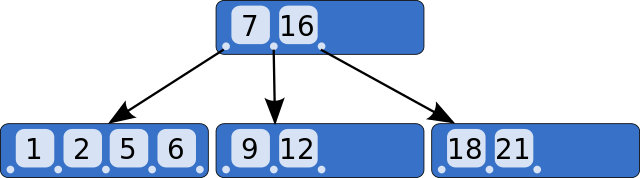
\includegraphics[width=.15\textwidth]{slides_images/b_tree_example}

\end{center}

\end{breakbox}

\begin{breakbox}
\boxtitle{Data Structure for Inverted Index}

Usually B-trees since they are sorted. Searching for a prefix like 'hyp\%' is now easier since the tree can just be traversed with h->y->p and then collect all children.
\end{breakbox}

\begin{breakbox}
\boxtitle{Blocked Sort-Based Indexing (BSBI)}

Problem of inverted index so far: parse docs one at a time => cannot exploit compression tricks. Solution: Blocked sort-based indexing. Try to keep data as compressed as possible.

\begin{itemize}
	\item External sorting algorithm
	\item Sorting with fewer disk seeks. Basic idea:
		\begin{itemize}
			\item Accumulate postings for each block, sort, write to disk
			\item Then merge the blocks into one long sorted order		
		\end{itemize}
	\item Problem: Keeps dictionary in memory
		\begin{itemize}
			\item Answer: Single-pass in-memory indexing
		\end{itemize}
\end{itemize}

\end{breakbox}